\documentclass[11pt,letterpaper]{article}
\usepackage[letterpaper,margin=0.75in]{geometry}
\usepackage[utf8]{inputenc}
\usepackage[T1]{fontenc}
\usepackage{hyperref}

%Hyperref format
\hypersetup{
	colorlinks=true,	% Hyperlinks are colored
	linkcolor=blue,		% Color of internal links (within document)
	citecolor=blue,	    % Color of internal links to the Reference page (within document)
	urlcolor=blue,		% Color of URLs (external) - default is magenta.
	pdftitle = {Predicting mechanical properties of FFF parts1},
	pdfsubject = {Prelim 2020},
	pdfauthor = {Gerardo A. Mazzei Capote},
	pdfkeywords = { },	
}
\usepackage{textcomp} % I think the bullet point shapes come from here
\usepackage[backend=bibtex, sorting=none,maxbibnames=99]{biblatex} %References are numbered per order of use in the text as opposed to alphabetically (default)
\addbibresource{BibTex/mypapers.bib}

\usepackage{tgpagella}% The headerrow command makes a table, this package
					  % Allows us to change the column seperation distance
\setlength{\tabcolsep}{0em} % Change the column seperation distance to 0em

\usepackage{enumitem} % Allows changing the spacing between items in a list
\setlist{nosep} % Change the spacing to zero

\usepackage{endnotes} % Enables the creation of end notes
\renewcommand{\notesname}{} % Remove the word "Notes" from the end notes
\let\enotesize\normalsize % Make endnotes the same size as document

% used for loading graphics
\usepackage{graphicx}
\graphicspath{{Figures/}}
% used for making sub-figures
\usepackage{subfig}
%used for placing text over images
\usepackage[percent]{overpic}

% Create a length variable for the table in skills. It is the text width
% minus the indent
\newlength{\skillswidth}
\setlength{\skillswidth}{\textwidth}
\addtolength{\skillswidth}{-\parindent}

% indentsection style, used for sections that aren't already in lists
% that need indentation to the level of all text in the document
\newenvironment{indentsection}[1]%
{\begin{list}{}%
	{\setlength{\leftmargin}{#1}}%
	\item[]%
}
{\end{list}}

% opposite of above; bump a section back toward the left margin
\newenvironment{unindentsection}[1]%
{\begin{list}{}%
	{\setlength{\leftmargin}{-0.5#1}}%
	\item[]%
}
{\end{list}}

% Create a headerrow command for the header of each skills section
\newcommand{\headerrow}[3]
{\vspace{0.4em}
\noindent
% To get the three items spaced left, center, right, I had to use this funny
% \extracolsep stuff. Got it working though.
\begin{tabular*}{\textwidth}{l @{\extracolsep{\fill}} cr}
	\textbf{#1} & % Title/Postion
	#2 &		  % Company Name
	\textbf{#3}\\ % Employment dates
\end{tabular*}}

%\usepackage{bibentry}
%\nobibliography*

% and the actual content starts here
\begin{document}


\begin{center}
	{\LARGE \textbf{Gerardo Andrés Mazzei Capote}}

	45 N. Randall Ave, Apt. 109\ \ \textbullet
	\ \ Madison, WI- 53715
	\\
	(608) 622-4643 \ \textbullet
	\ \ mazzeicapote@wisc.edu\\
	\href{https://www.linkedin.com/in/gerardo-mazzei-capote}{linkedin.com/in/gerardo-mazzei-capote}
	
\end{center}
\vspace{-0.5em}
\hrule
\vspace{0.4em}
\vspace{-1em}

\section*{PORTFOLIO}

Fused Filament Fabrication (FFF), also known as Fused Deposition Modeling (FDM), is arguably the most widely available Additive Manufacturing (AM) technology at the moment. Offering the possibility of producing complex geometries in a compressed product development cycle and in a plethora of materials, it comes as no surprise that FFF is attractive to multiple industries, including the automotive and aerospace segments. However, the high anisotropy of parts developed through this technique imply that part failure prediction is extremely difficult \textemdash a requirement that must be satisfied to guarantee the safety of the final user. This pain point represents one of the major factors currently hindering the adoption of FFF and other AM technologies as legitimate manufacturing techniques, given that the safety of the final product is hard to guarantee since the failure behavior of the object is difficult to assess. The research I have conducted during my graduate studies is aimed at solving this issue by estimating the likelihood of part failure through a mathematical model, known as a Failure Criterion (FC), that allows engineers to safely assess if a given FFF part will hold its structural integrity considering its intended application. Calculation of the FC parameters requires destructive testing of coupons, produced with a variety of orientations of the deposited polymer strands during printing, traditionally referred to in literature as the bead orientation.

The lack of standardization in the field of AM posed a challenge: it was a necessity to develop customized specimen geometries, mechanical testing protocols, as well as the extrusion of a customized FFF filament produced with tight geometrical constraints and controlled production parameters that ensured that fluctuations in the material dimensions and quality would not introduce lurking variables into the experiments. Additionally, some of the required bead orientations necessary to fully describe the failure function were unattainable through the use of a traditional FFF printer, requiring the deployment of custom toolpath solutions using a unique 6-axis 3D printer developed in the Polymer Engineering Center at the University of Wisconsin-Madison.

\begin{figure}[h]
	\center
	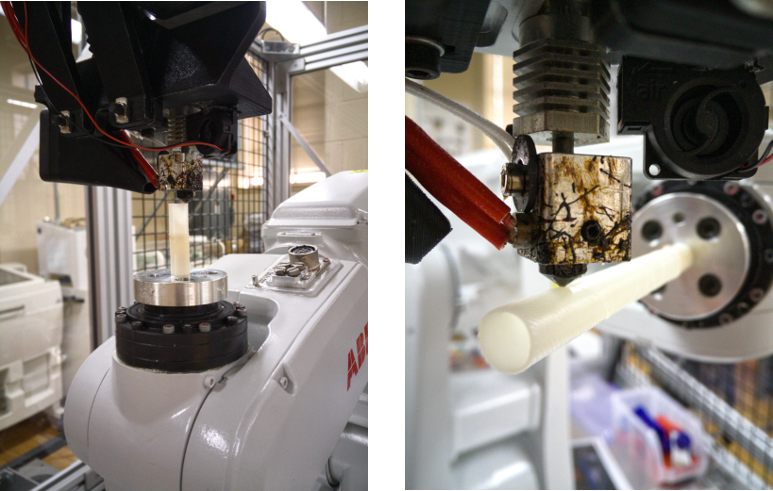
\includegraphics[height=6cm, keepaspectratio]{otto2}
	\captionsetup{justification=centering} %long caption
	\caption[6-axis printer]{6-axis printer mid-print.} \label{fig:otto2}
\end{figure}    

The resulting failure model has been proven to be capable of accurately capturing the failure behavior of FFF parts, as shown by experimental work where the predicted catastrophic failure stress of an FFF part tested in tension was within 10\% of the real failure stress. This has in turn allowed the FC and the methodology derived within this research project to be used to predict part failure in other AM techniques, such as Selective Laser Sintering (SLS) and Multi-Jet Fusion (MJF). Future research is aimed at streamlining the process through machine learning algorithms and minimization of the required mechanical tests necessary to populate the FC function.

\begin{figure}[!htbp]
	\center
	\includegraphics[width=\linewidth, keepaspectratio]{final_surface}
	\captionsetup{justification=centering} %long caption
	\caption[Complete Failure Surface]{Complete Failure Surface plotted with calculated f values of 1, 0.75, 0.50 and 0.25 to illustrate safety factors of 1, 4/3, 2 and 4 respectively.} \label{fig:fullfs}
\end{figure}


This research project has led to three peer reviewed publications, three technical presentations in important AM conferences (SFF, RAPID, AMUG), and international collaborations with renowned institutes such as the Technical University of Munich (TUM), the National School of Engineers of Saint-\'Etienne (ENISE), as well as contributions with industry partners such as BMW and Netzsch.


Additional research venues pursued during my graduate studies included the following short term projects:
\begin{enumerate}
	\item Development and construction of a low-cost, reusable N9X mask during the COVID19 pandemic. Effort awarded with financial support from the Wisconsin Alumni Research Foundation (WARF).
	\item Extrusion of a Polyethylene Terephthalate (PET) FFF filament produced using discarded bottles as the parent material.
	\item Fabrication of Heat Exchanger units (HX) manufactured through polymer AM techniques.
\end{enumerate}

\end{document}
